‫\section*{پیاده‌سازی \lr{Cache Replacement Imitating Belady's OPT Policy} در \lr{Gem5}}
‫\subsection*{صورت پروژه}
‫در این پروژه قصد داریم طبق \href{https://www.cs.utexas.edu/~lin/papers/hpca22.pdf}{این مقاله} یک سیاست جایگزینی حافظه نهان را به \lr{Gem5} اضافه کنیم و با اجرای یک برنامه محک، آن را با سیاست‌های موجود مقایسه کنیم.
‫\subsection*{سیاست جایگزینی معرفی شده در مقاله}
‫ابتدا فاصله زمانی استفاده مجدد هر خط در حافظه پیش‌بینی می‌شود و سپس خطوط بر اساس زمان پیش‌بینی شده استفاده مجددشان حذف می‌شوند.
‫\subsection*{گام‌های پروژه}
‫\شروع{شمارش}
‫\فقره توضیح دادن چگونگی عملکرد این سیاست جاگزینی، پیچیدگی پیاده‌سازی آن به صورت سخت‌افزاری و هزینه پیاده‌سازی در گزارش
‫\شروع{فقرات}
‫\فقره آریان افضل‌زاده
‫\فقره فاطمه حمدی
‫\پایان{فقرات}
‫\فقره ایجاد سیاست مد نظر در این پروژه در \lr{Gem5}
‫\شروع{فقرات}
‫\فقره تمامی اعضای گروه
‫\پایان{فقرات}
‫\فقره افزودن سیاست ایجاد شده به سیاست‌های پیش‌فرض \lr{Gem5}
‫\شروع{فقرات}
‫\فقره آریان افضل‌زاده
‫\پایان{فقرات}
‫\فقره شبیه‌سازی سه برنامه محک و مقایسه‌ی عملکرد این سیاست با سیاست‌های \lr{LRU} و \lr{LFU}
‫\شروع{فقرات}
‫\فقره ملیکا علی‌زاده
‫\فقره الینا هژبری
‫\پایان{فقرات}
‫\فقره نوشتن یک اسکریپت پایتون که ده برنامه محک مختلف را روی این سیاست و چهار سیاست معروف شبیه‌سازی کند و نتایج شبیه‌سازی را در قالب چند نمودار و یک فایل با فرمت CSV ارائه دهد
‫\شروع{فقرات}
‫\فقره فاطمه حمدی
‫\فقره ملیکا علی‌زاده
‫\فقره الینا هژبری
‫\پایان{فقرات}
‫\پایان{شمارش}
‫\newpage
‫\section*{چکیده مقاله}
‫در این پروژه می خواهیم سیاست \lr{Belady's MIN} را پیاده سازی کنیم. طبق مقاله این سیاست باید به آخرین سطح \lr{cache} اعمال شود تا خطی که پیش بینی شده در آینده دوباره استفاده می شود را خارج کند.
‫ زمان تقریبی رسیدن به هر خط \lr{(ETA)} برابر جمع زمان کنونی و پارامتری به اسم \lr{Predicted Reuse Distance} است. در هر درج خط با بزرگترین \lr{ETA} خارج می شود. همچنین برای پیش بینی \lr{reuse distance} از یک پیش بینی کننده بر اساس \lr{PC} استفاده می شود تا \lr{reuse distance} هر خط \lr{cache} تخمین زده شود.
‫ این سیاست سه جز اصلی دارد:\\
‫1. \lr{Sample Cache}\\
‫2. \lr{Reuse Distance Predictor(RDP)}\\
‫3. \lr{ETA Counter}\\
‫\begin{description}
‫\item[\lr{Sample Cache}] \end{description}
‫به طور خلاصه این جز \lr{reuse distance} های قبلی را برای \lr{train} کردن \lr{RDP} استفاده می کند. برای این کار یک تاریخچه با اندازه 8 برابر نمونه برداشته شده دارد که دسترسی های منحصر به فرد گذشته \lr{cache} را نگه می دارد.
‫\begin{description}
‫\item[\lr{RDP}] \end{description}
‫یک پیش بینی کننده بر اساس \lr{PC} است که \lr{reuse distance} را برای ورودی هایی که توسط \lr{PC}وارد می شوند، یاد می گیرد. هر ورودی در \lr{RDP}، 0 مقداردهی می شود و با استفاده مجدد هر خط در \lr{sample cache} ورودی \lr{RDP} مربوط به \lr{PC} که آخرین بار به خط دسترسی داشته، با استفاده از \lr{reuse distance} مشاهده شده به روز می شود.
‫چون مقدار \lr{reuse distance} برای \lr{PC} ممکن است نوسان کند، از پارامتری به اسم \lr{temporal difference learning} (مقادیر پیش بینی شده را به روز می کند به عنوان یک تابع خطی از تفاوت بین مقادیر پیش بینی شده و مشاهده شده) برای آموزش \lr{RDP} استفاده می کند .\\
‫به طور کلی ورودی های \lr{RDP} به این صورت \lr{train}  می شود که اگر \lr{reduce distance} جدید از مقدار قبلی بزرگتر بود مقدار ورودی با \lr{W} جمع زده می شود و اگر کوچکتر بود، مقدار ورودی منهای \lr{w} می شود. همچنین اگر وجود نداشت، ورودی به عنوان \lr{reuse distance} ست می شود.
‫\\\[diff=absolute\: difference\: between\: the\: previous\: entry\: and\: the\: new\: reuse\: distance\]
‫\[w=min(1, \frac{diff}{16})\]
‫\begin{description}
‫\item[\lr{ETA counters}] \end{description}
‫در نهایت خود \lr{cache} ، \lr{ETA} را برای هر خط حفظ می کند. پس از درج در حافظه نهان، فاصله استفاده مجدد پیش بینی شده خط به یک \lr{ETA} تبدیل می شود و این مقادیر \lr{ETA} برای تصمیم کیری برای خروج از حافظه پنهان آینده استفاده می شود. درج های \lr{cache} که پیش بینی می شود مقادیر \lr{ETA} بزرگتر از هر خط موجود در مجموعه داشته باشند، دور زده می شوند، به این معنی که در حافظه پنهان درج نمی شوند.
‫\begin{description}
‫\item[\lr{Estimated Time Remaining (ETR)}] \end{description} برای کاهش هزینه نگهداری \lr{time stamp} های دقیق \lr{ETA} برای هر خط \lr{cache}، از یک مقدار کوچکتر اما منطقاً معادل، به نام \lr{Estimated Time Remaining (ETR)}  استفاده می‌شود. مقدار \lr{ETR} با \lr{predicted reuse distance} خط مقدار دهی اولیه می‌شود و هر بار که به خط دیگری در مجموعه دسترسی پیدا می‌شود، کاهش می‌یابد. با کاهش تفاوت بین زمان حال و \lr{ETA} پیش بینی شده یک خط \lr{cache}،  \lr{ETR} آن خط نیز کاهش می یابد. بنابراین، ترتیب نسبی \lr{ETR} ها دقیقاً مشابه ترتیب نسبی \lr{ETA} ها است.\\\begin{description}
‫\item[\lr{Handling Imprecise Predictions}] \end{description}
‫ گاهی اوقات، سیستم ممکن است \lr{reuse distance} یک خط را دست‌کم بگیرد و باعث شود مقدار شمارنده \lr{ETR} آن بدون مشاهده \lr{reuse} به 0 برسد. اگر مقدار شمارنده در 0 اشباع شود، این خط همیشه بالاترین اولویت ذخیره سازی را حفظ می کند که نامطلوب است. برعکس، اگر به چنین خطوطی یک مقدار \lr{ETR} بی نهایت داده شود، آنگاه خطوطی که \lr{ETA} آنها فقط با مقدار کمی دست کم گرفته شده است، بلافاصله خارج می شوند، که این نیز نامطلوب است. برای رسیدگی به این پیش‌بینی‌های غیردقیق، سیستم پس از رسیدن به مقدار 0، شمارنده‌های \lr{ETR} را کاهش می‌دهد. به عنوان مثال،  \lr{ETR counter} با مقدار \lr{-4}  نشان می دهد که خط با 4 دسترسی مجموعه ای از \lr{ETA} خود فراتر رفته است. پس از اخراج، این سیاست، خطی را با بزرگترین مقدار مطلق \lr{ETR}، که دورترین خط از \lr{ETA} آن است، خارج می کند. بنابراین، خط اخراج شده یا پیش‌بینی می‌شود که در آینده بیشتر مورد استفاده مجدد قرار گیرد یا در گذشته پیش‌بینی می‌شود که در دورترین فاصله‌ها مورد استفاده مجدد قرار گیرد. پیوندها با بیرون کردن خطوط با \lr{ETR}  منفی به نفع خطوط با \lr{ETR} مثبت شکسته می شوند.
‫\newpage
‫\section*{بخش امتیازی}
‫در این بخش ابتدا 10 برنامه محک را به صورت رندم \lr{generate} کردیم، برای این که بتوانیم این 10 برنامه را با استفاده از 4 سیاست مختلف روی \lr{gem5} شبیه سازی کنیم، باید مراحل زیر را انجام دهیم تا قابلیت سیاست حافظه نهان اضافه شود :\\
‫ابتدا باید قابلیت سیاست جایگزینی را اضافه کنیم، پس در فایل \lr{configs/common/ObjectList.py} خط زیر را اضافه می کنیم:\\
‫\lr{repl-list = ObjectList(getattr(m5.objects , "BaseReplacementPolicy", None))}
‫سپس در فایل \lr{configs/common/Options.py} به تابع \lr{addNoISAOptions} باید کد زیر را اضافه کنیم:\\
‫\lr{parser.add-argument("--l2-repl", default="LRURP",
‫    choices=ObjectList.repl-list.get-names(),
‫    help = "replacement policy for l2")}\\
‫    سپس در فایل \lr{configs/common/ CacheConfig.py} به تابع \lr{-get-cache-opts} کد زیر را اضافه می کنیم:\\
‫    \lr{replacement-policy-attr = f"{level}-repl"
‫    if hasattr(options , replacement-policy-attr): opts["replacement policy"] = \\ObjectList.repl-list.get(getattr(options ,replacement policy-attr))()}\\
‫حال اگر در هنگام شبیه سازی دستور \lr{-l2-repl} را بزنیم می توانیم نوع سیاست جایگزینی را 
‫ مشخص کنیم و شبیه سازی را طبق آن انجام دهیم. در اینجا نیازی به ساخت فایل کانفیگ نیست و می توان 
‫ از فایل پیش فرضی که در آدرس \lr{configs/deprecated/example/se.py} است، استفاده کنیم.\\
‫حال از یک اسکریپت پایتون برای اجرای این برنامه ها با سیاست های مختلف استفاده می کنیم به این صورت 
‫که ابتدا در یک حلقه تمامی فایل های محک را به فایل باینری تبدیل می کنیم به کمک دستور زیر:\\
‫\lr{gcc -o tests/test tests/test.c}\\
‫سپس تمام سیاست های مورد نظر را در یک آرایه قرار می دهیم و با زدن حلقه روی این فایل های باینری و سیاست ها تمام فایل ها را روی سیاست های مختلف اجرا می کنیم. در اصل از دستور زیر استفاده شده:\\
‫\lr{./build/X86/gem5.opt configs/deprecated/example/se.py -c tests/test --caches --l2cache --l2-size=4kB --mem-type=DDR4-2400-16x4 --cacheline-size 128 --cpu-type=TimingSimpleCPU --l2-repl=LRURP}\\
‫حال اطلاعات شبیه سازی این برنامه ها که در فایل \lr{stats.txt} ذخیره شده است را داریم و اطلاعاتی مثل \lr{CPI} و \lr{miss rate} را از آن ها خوانده و در فایل \lr{csv} ذخیره می کنیم. سپس با استفاده از این اطلاعات نمودار های مربوط به هر برنامه محک را با تفکیک سیاست ها رسم می کنیم.\\
‫‫‫‫‫‫‫‫‫‫‫‫‫‫‫‫‫‫‫‫‫‫‫‫‫‫‫‫‫‫‫‫‫‫‫‫‫‫‫‫‫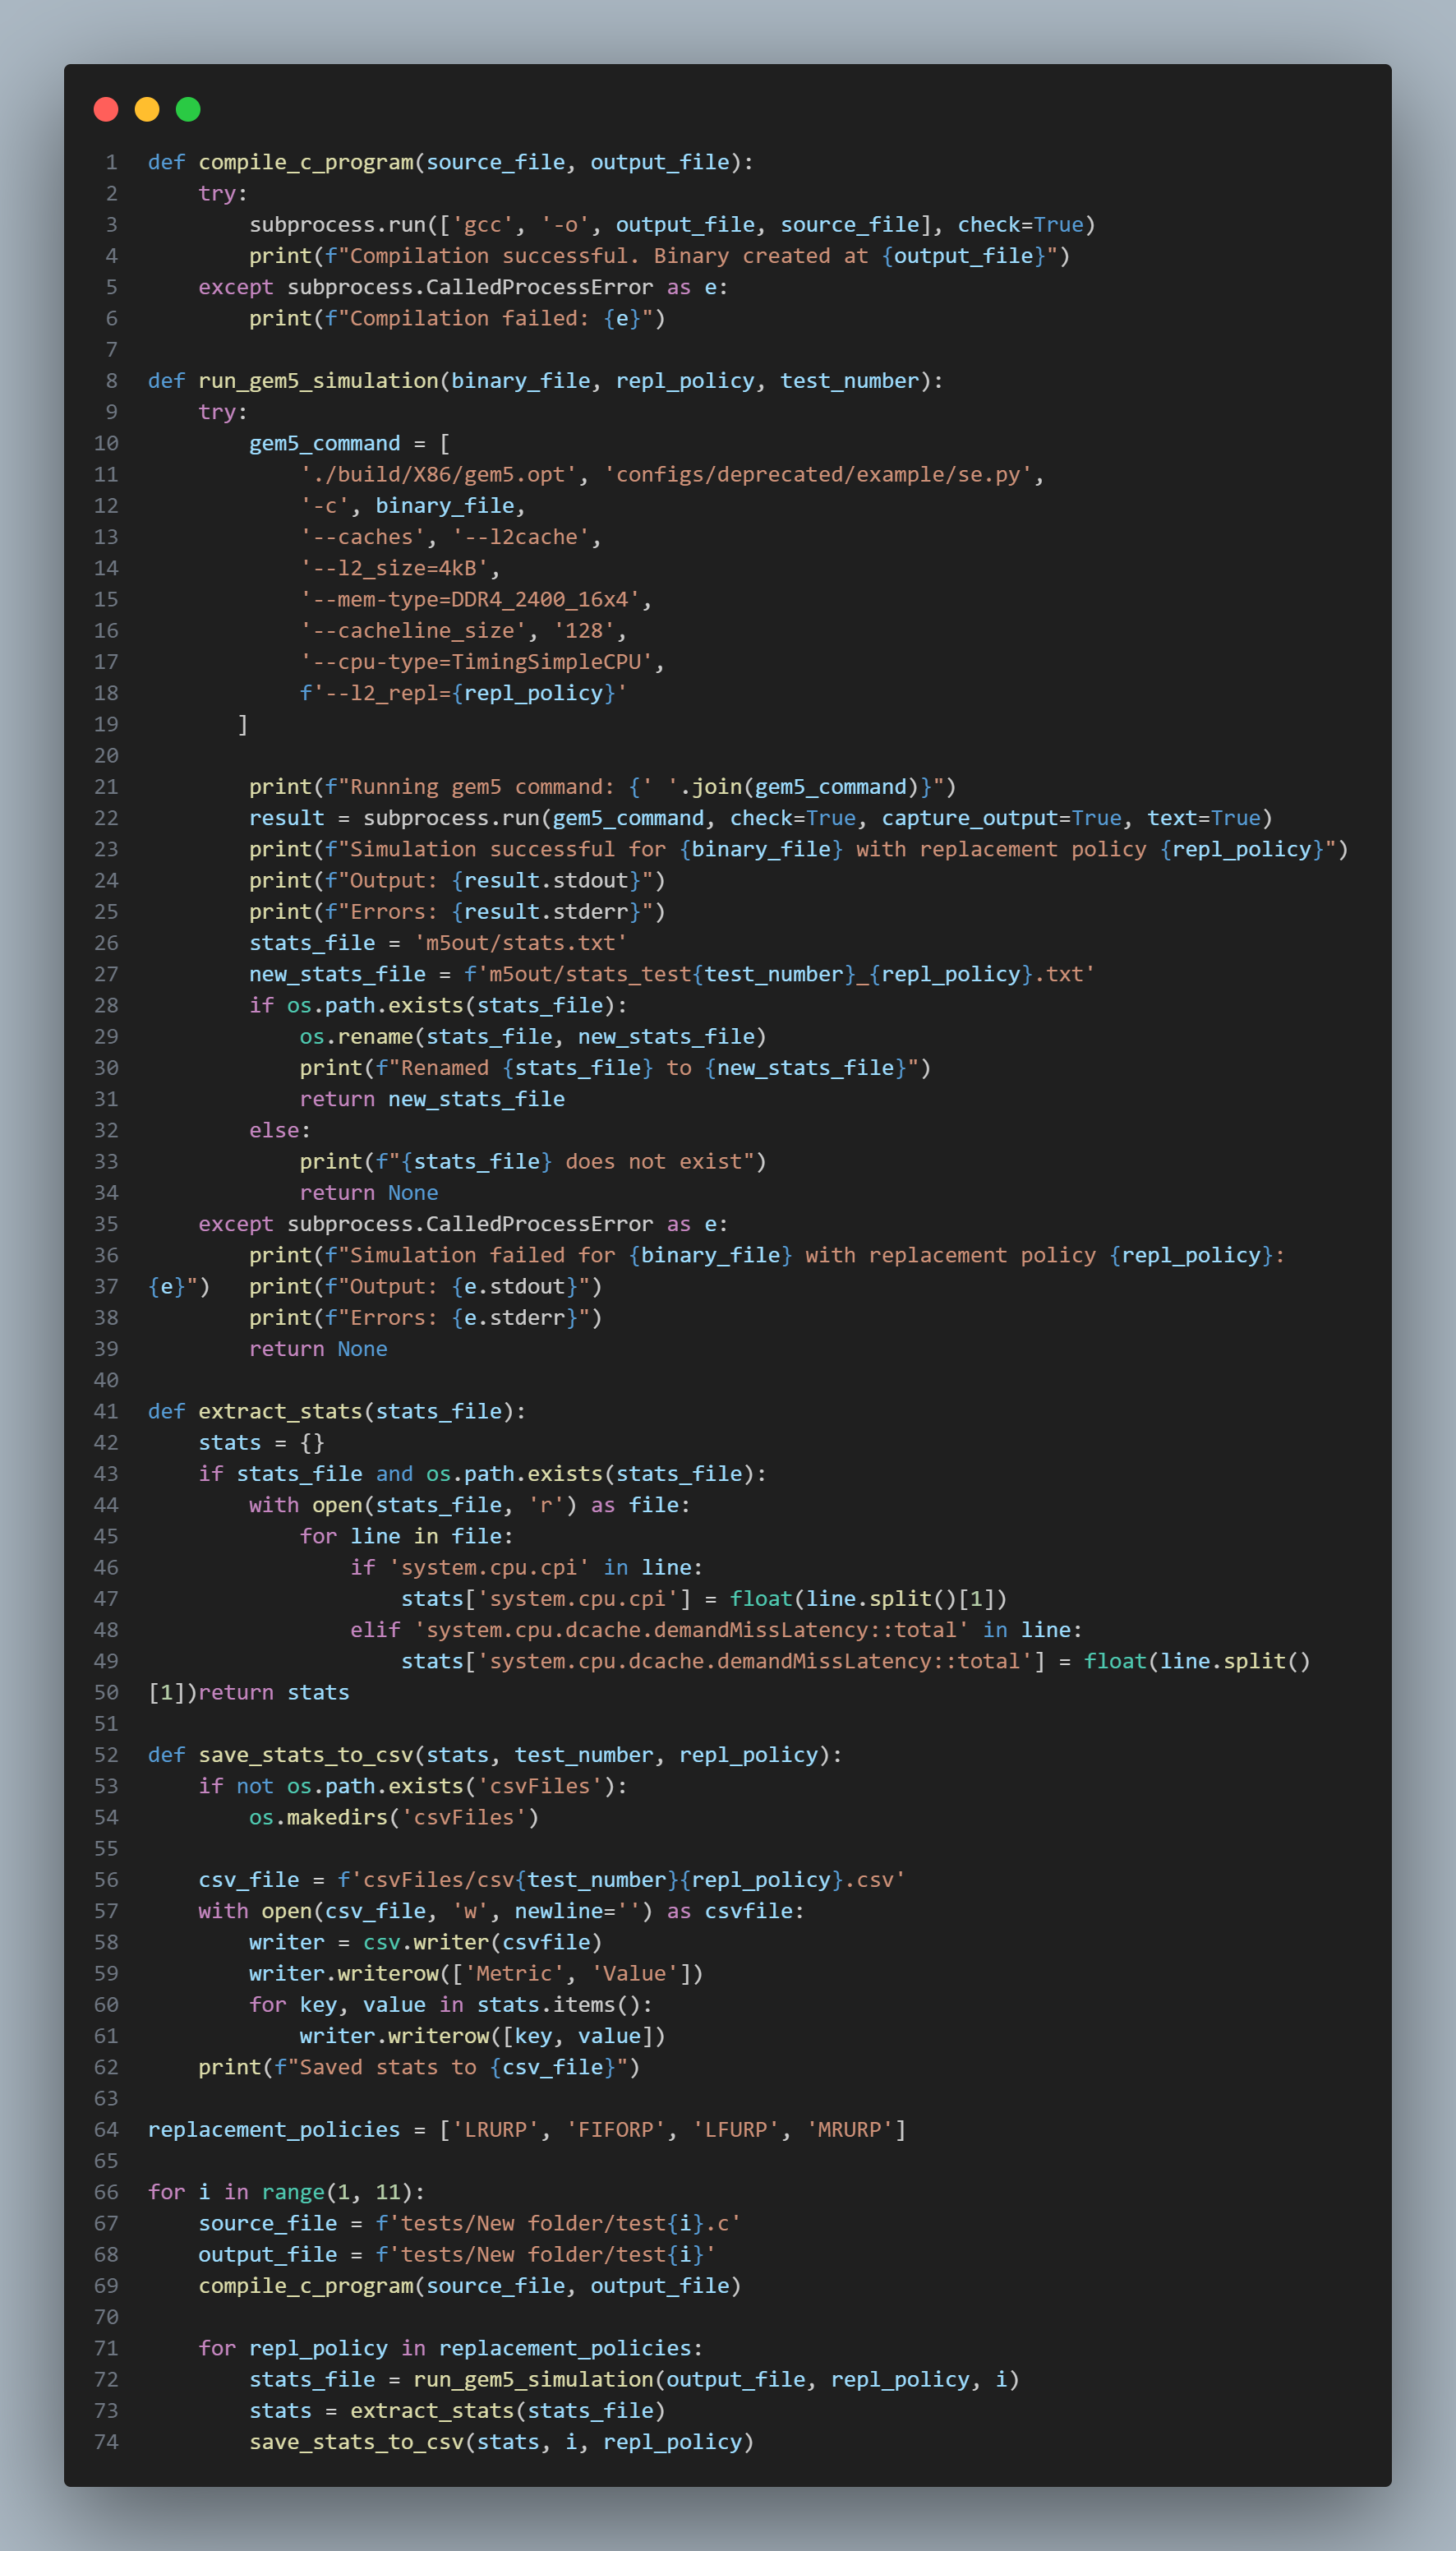
\includegraphics[width=0.8\textwidth]{code.png}\newpage
‫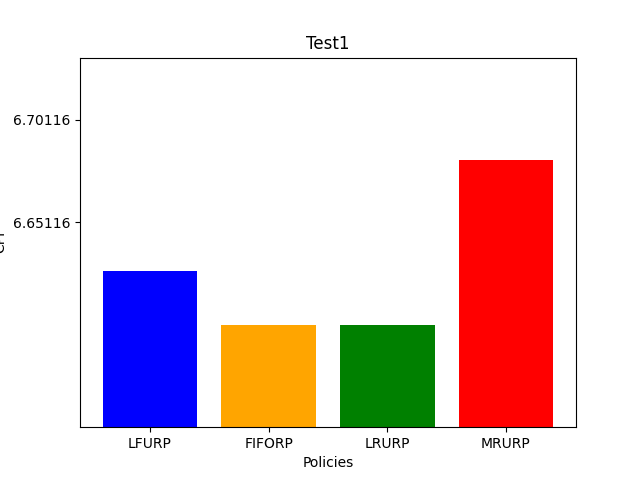
\includegraphics[width=0.8\textwidth]{graph/csv1CPI.png}\\
‫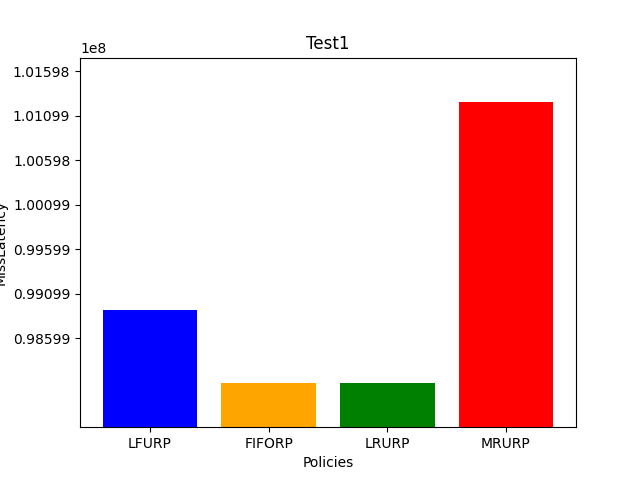
\includegraphics[width=0.8\textwidth]{graph/csv1Miss.png}\\
‫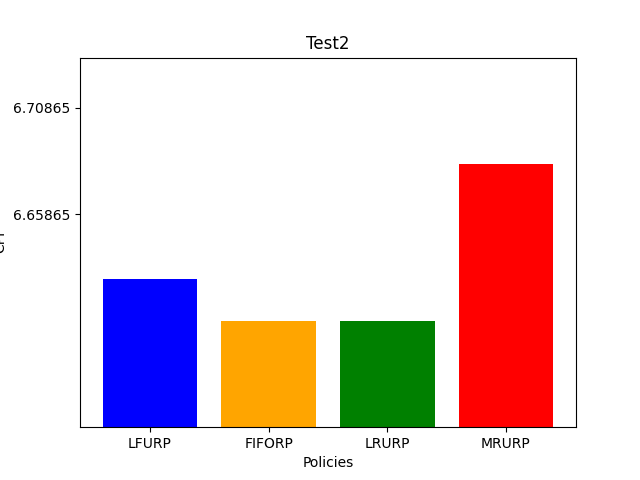
\includegraphics[width=0.8\textwidth]{graph/csv2CPI.png}\\
‫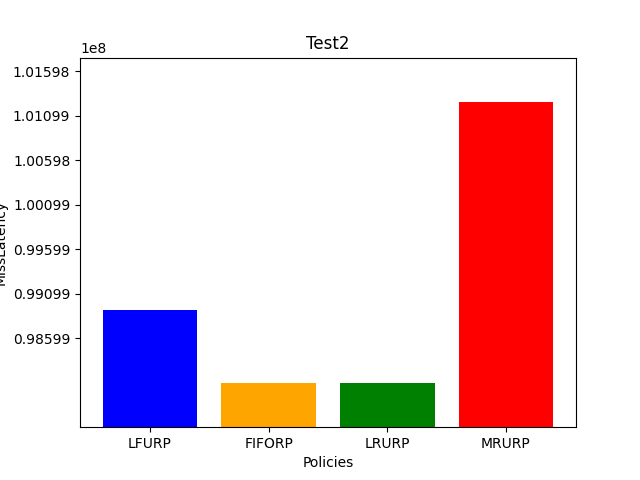
\includegraphics[width=0.8\textwidth]{graph/csv2Miss.png}\\
‫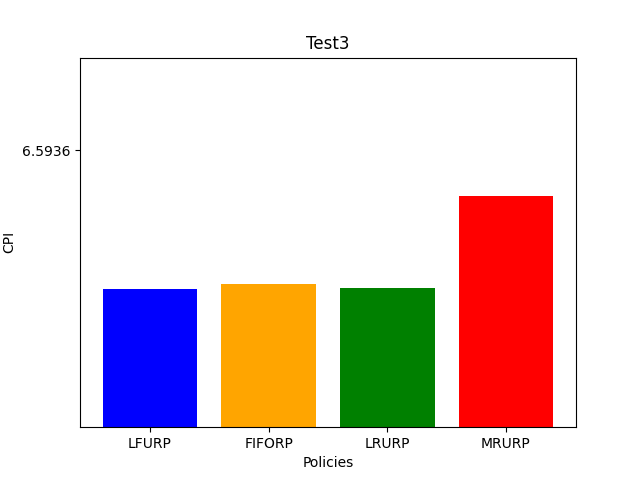
\includegraphics[width=0.8\textwidth]{graph/csv3CPI.png}\\
‫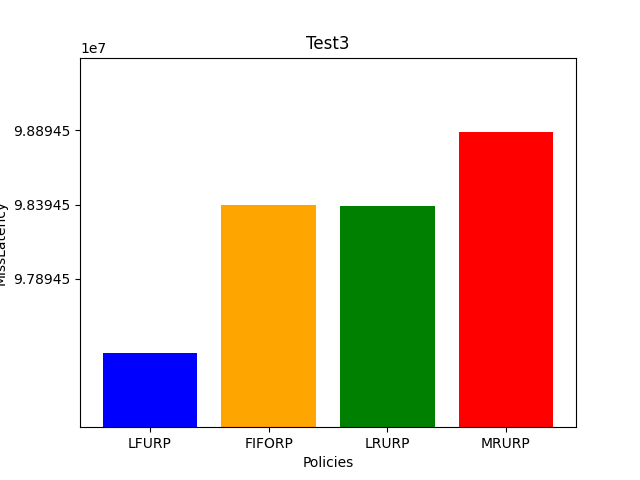
\includegraphics[width=0.8\textwidth]{graph/csv3Miss.png}\\
‫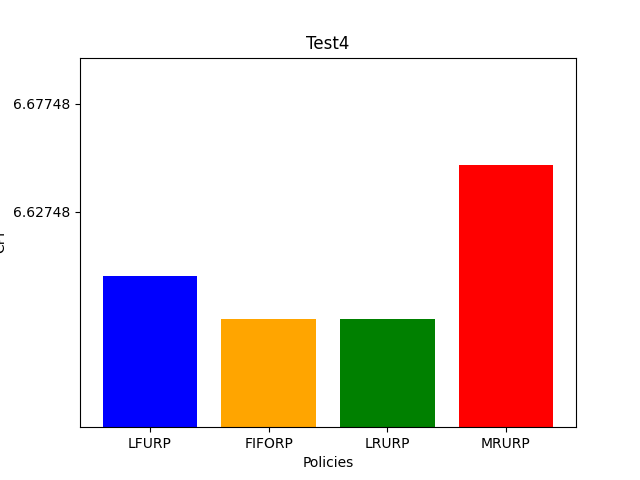
\includegraphics[width=0.8\textwidth]{graph/csv4CPI.png}\\
‫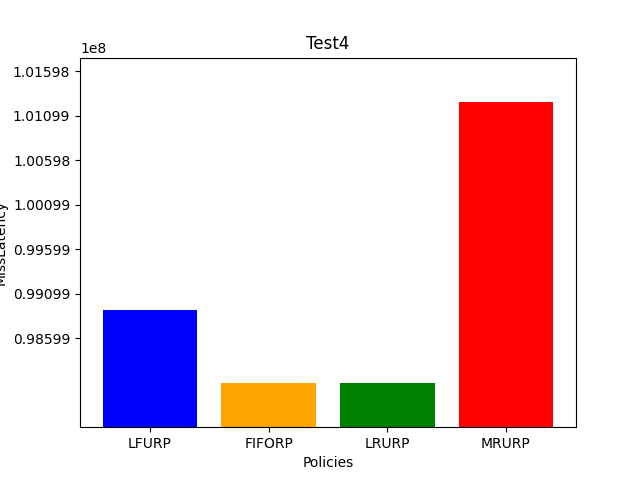
\includegraphics[width=0.8\textwidth]{graph/csv4Miss.png}\\
‫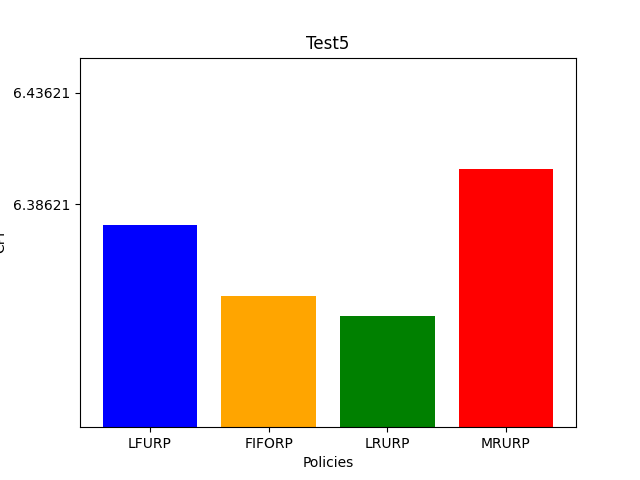
\includegraphics[width=0.8\textwidth]{graph/csv5CPI.png}\\
‫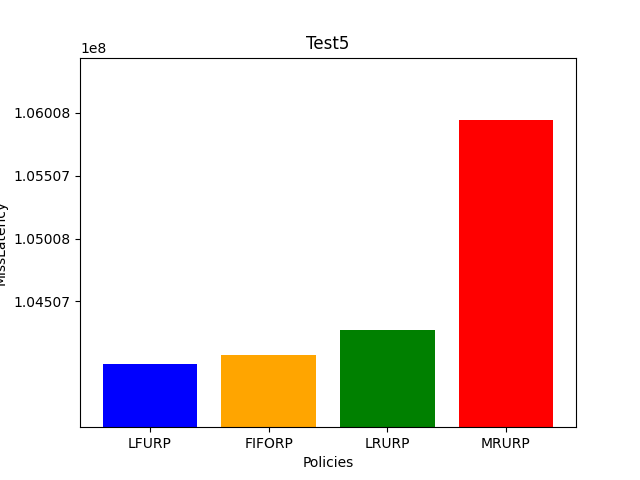
\includegraphics[width=0.8\textwidth]{graph/csv5Miss.png}\\
‫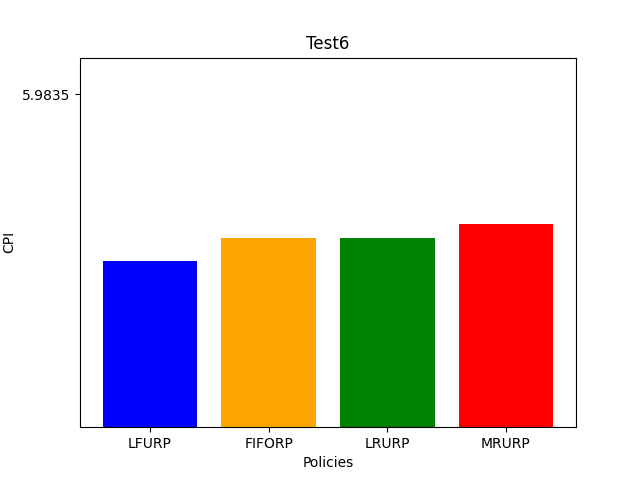
\includegraphics[width=0.8\textwidth]{graph/csv6CPI.png}\\
‫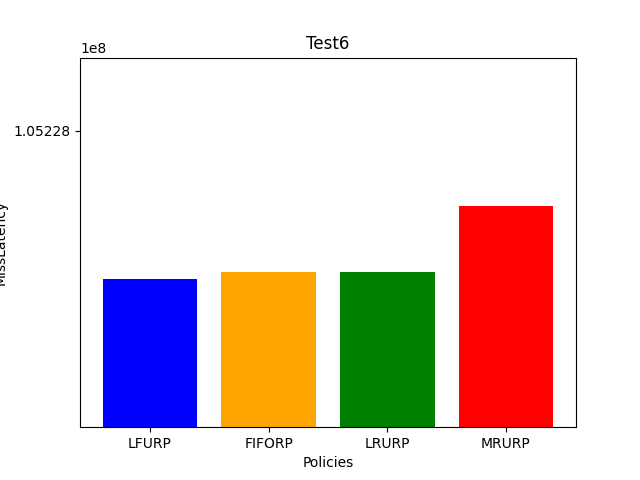
\includegraphics[width=0.8\textwidth]{graph/csv6Miss.png}\\
‫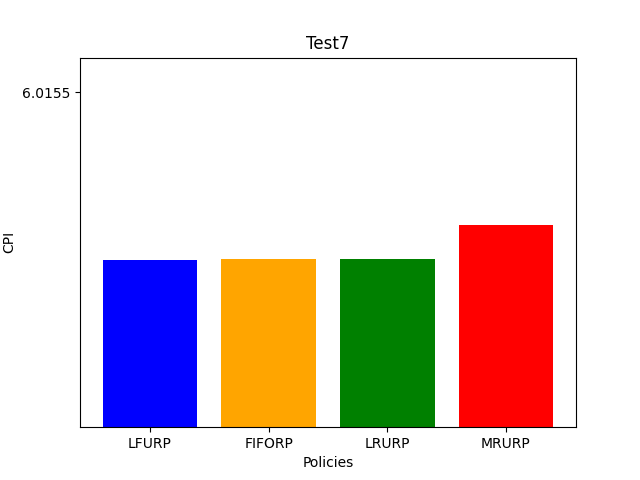
\includegraphics[width=0.8\textwidth]{graph/csv7CPI.png}\\
‫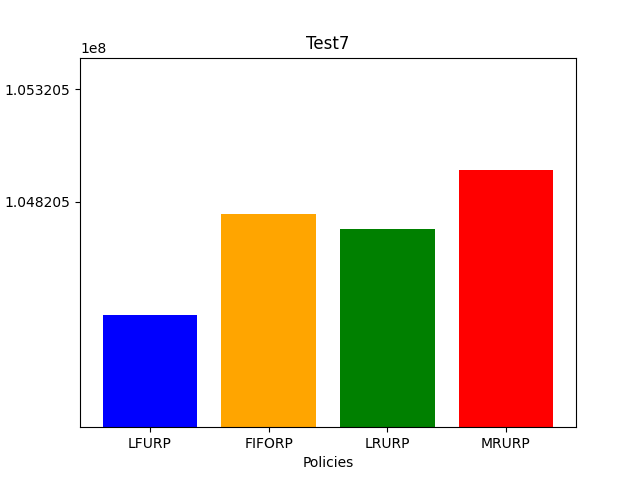
\includegraphics[width=0.8\textwidth]{graph/csv7Miss.png}\\
‫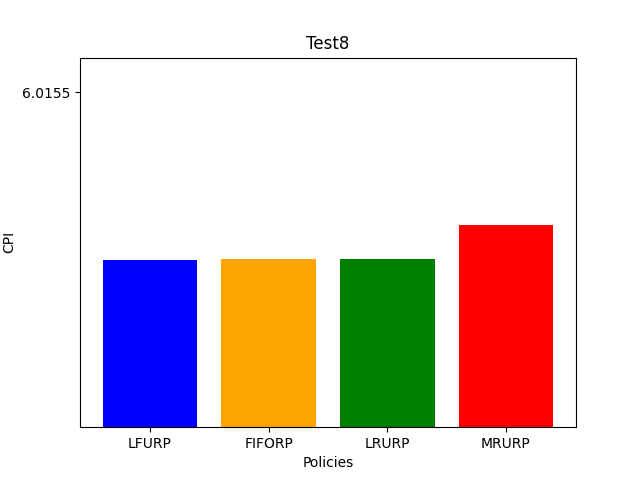
\includegraphics[width=0.8\textwidth]{graph/csv8CPI.png}\\
‫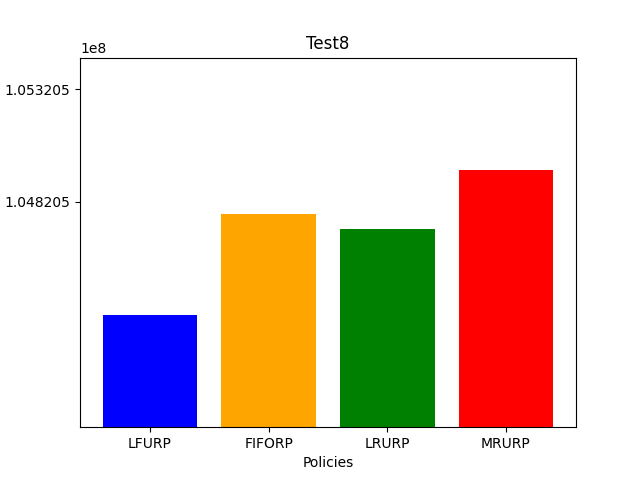
\includegraphics[width=0.8\textwidth]{graph/csv8Miss.png}\\
‫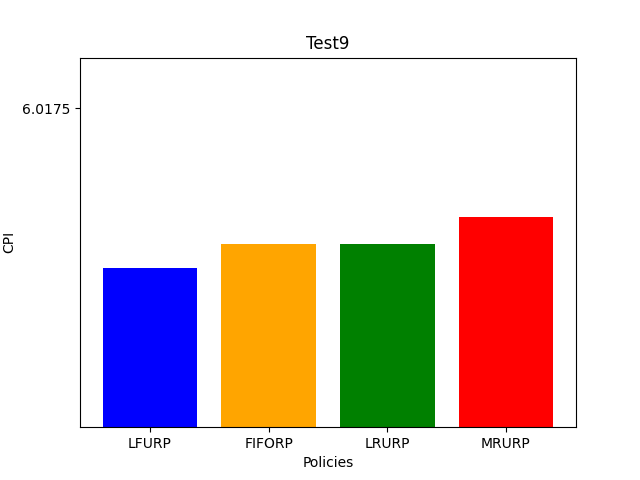
\includegraphics[width=0.8\textwidth]{graph/csv9CPI.png}\\
‫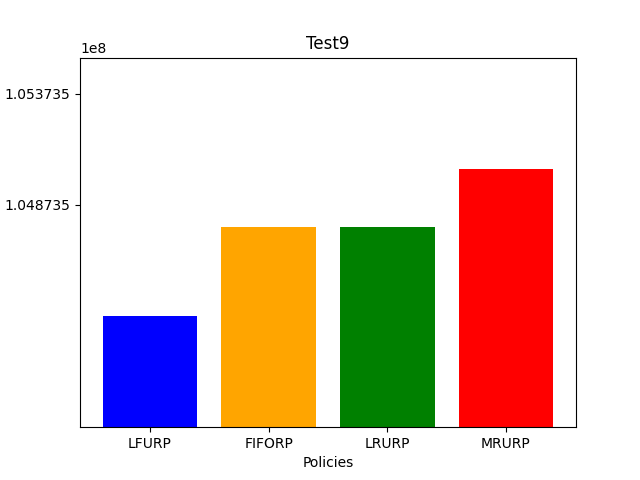
\includegraphics[width=0.8\textwidth]{graph/csv9Miss.png}\\
‫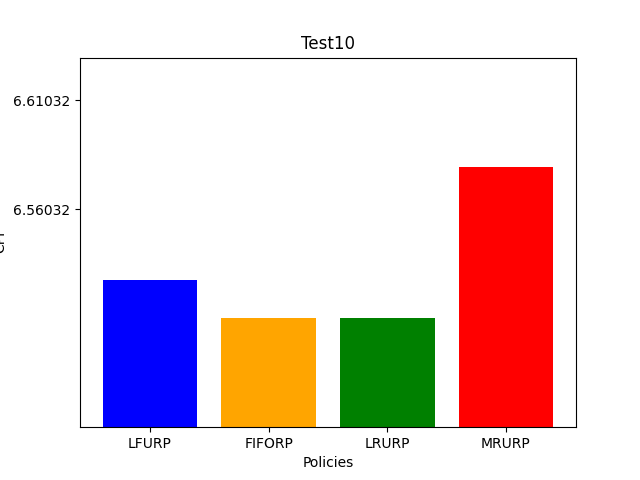
\includegraphics[width=0.8\textwidth]{graph/csv10CPI.png}\\
‫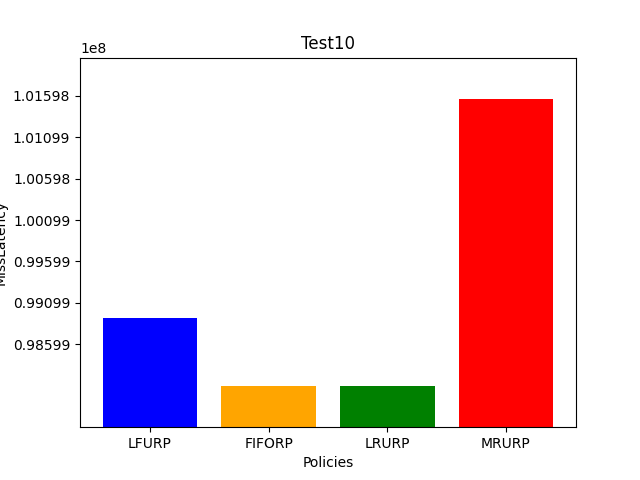
\includegraphics[width=0.8\textwidth]{graph/csv10Miss.png}\\